\documentclass{article}
\usepackage[latin1]{inputenc}
\usepackage[margin=1.0in]{geometry}
\usepackage{fancyhdr}
\usepackage{amsmath}
\usepackage{graphicx}
\usepackage{float}
\setcounter{secnumdepth}{2}
\setcounter{equation}{0}

\title{Kanto Player \\
CSEE W4840 Final Report}
\author{
  Kavita Jain-Cocks\\
  \texttt{kj2264@columbia.edu}
  \and
  Howard Mao\\
  \texttt{zm2169@columbia.edu}
  \and
  Amrita Mazumdar\\
  \texttt{am3210@columbia.edu}
  \and
  Darien Nurse\\
  \texttt{don2102@columbia.edu}
  \and
  Jonathan Yu\\
  \texttt{jy2432@columbia.edu}
   \\}
 \date{\today}
\begin{document}

\maketitle
\newpage

\abstract{This project presents an audio player with frequency visualization. 
The user is able to play audio files from an SD card and view a nice visualization 
on a VGA display. We use a field-programmable gate array (FPGA) for implementation, 
with software handling user interaction and song coordination and hardware handling 
actual audio output and FFT visualization. }

\section{Introduction}

\section{System Architecture}

\subsection{High-Level Overview}
% include data path
% block diagram

\section{Design Implementation}
\subsection{FFT Unit}
The FFT unit is used to compute the discrete frequency transform of a set of audio
samples to be visualized. 

\subsubsection{Fast Fourier Transform Algorithm}
We use the basic Cooley-Tukey FFT algorithm with a radix of 16 to compute the
frequency transform of a given sample. The number of frequencies \(N\) computed by 
the FFT was chosen to be 256. The radix size and number of frequencies were chosen 
to optimize for space and time. The basic DFT is defined by the equation:

\begin{equation}
	X_k = \sum_{n=0}^{N-1} x_n e^{-\frac{2\pi j}{N} nk}
\end{equation}

where \(k\) and \(n\) are integers from 0 to \(N\). 

According to the Cooley-Tukey algorithm, 
we split our original input into 16 different parts and perform a DFT on each
individual component. We can then recombine the individual DFT outputs in 4
recombination stages, using the following equation for each stage: 

\begin{equation}
	X_k = \left\{
	\begin{matrix}
		E_k + e^{-\frac{2\pi j}{N}k} O_k		& 	\mbox{if } k < N/2 \\ 
		E_{k-N/2} - e^{-\frac{2\pi j}{N} (k-N/2)} O_{k-N/2} & 	\mbox{if }
		k \geq N/2. 
	\end{matrix} 
	\right.
\end{equation}

The resulting output is 256 frequency values.

\newpage

\subsubsection{Block Diagrams}

The FFT hardware consists of two types of pipelines, one for the DFT,
and another for the recombination. 

\begin{figure}[H]
	\centering
	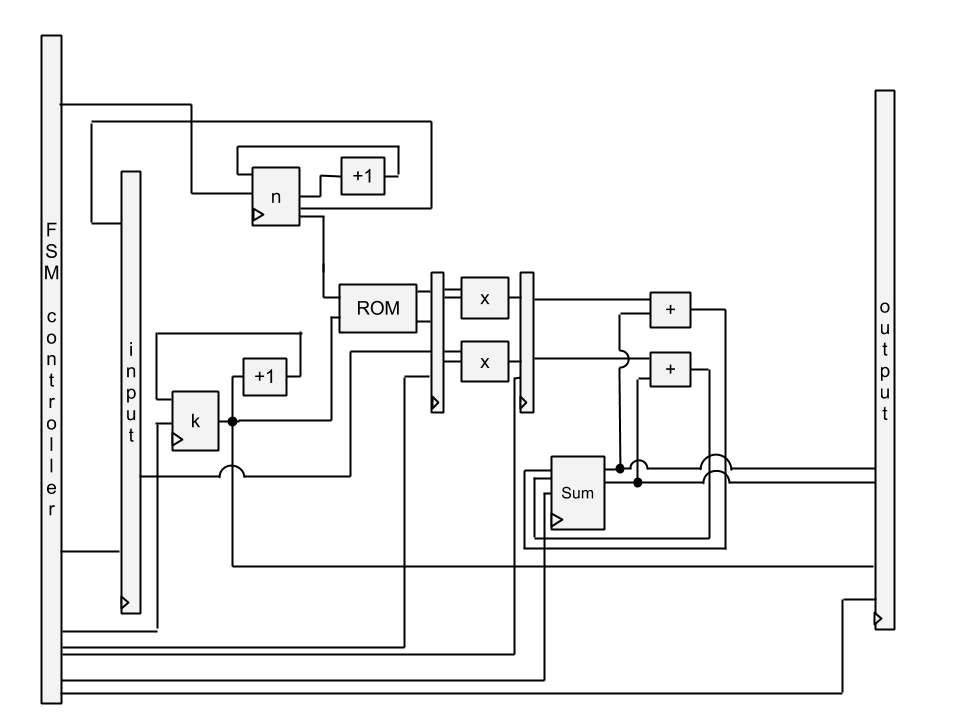
\includegraphics[scale=0.3]{dft-unit}
	\caption{DFT Unit}
\end{figure}

The DFT pipeline computes a 16-point DFT according to equation 1. 

\begin{figure}[H]
	\centering
	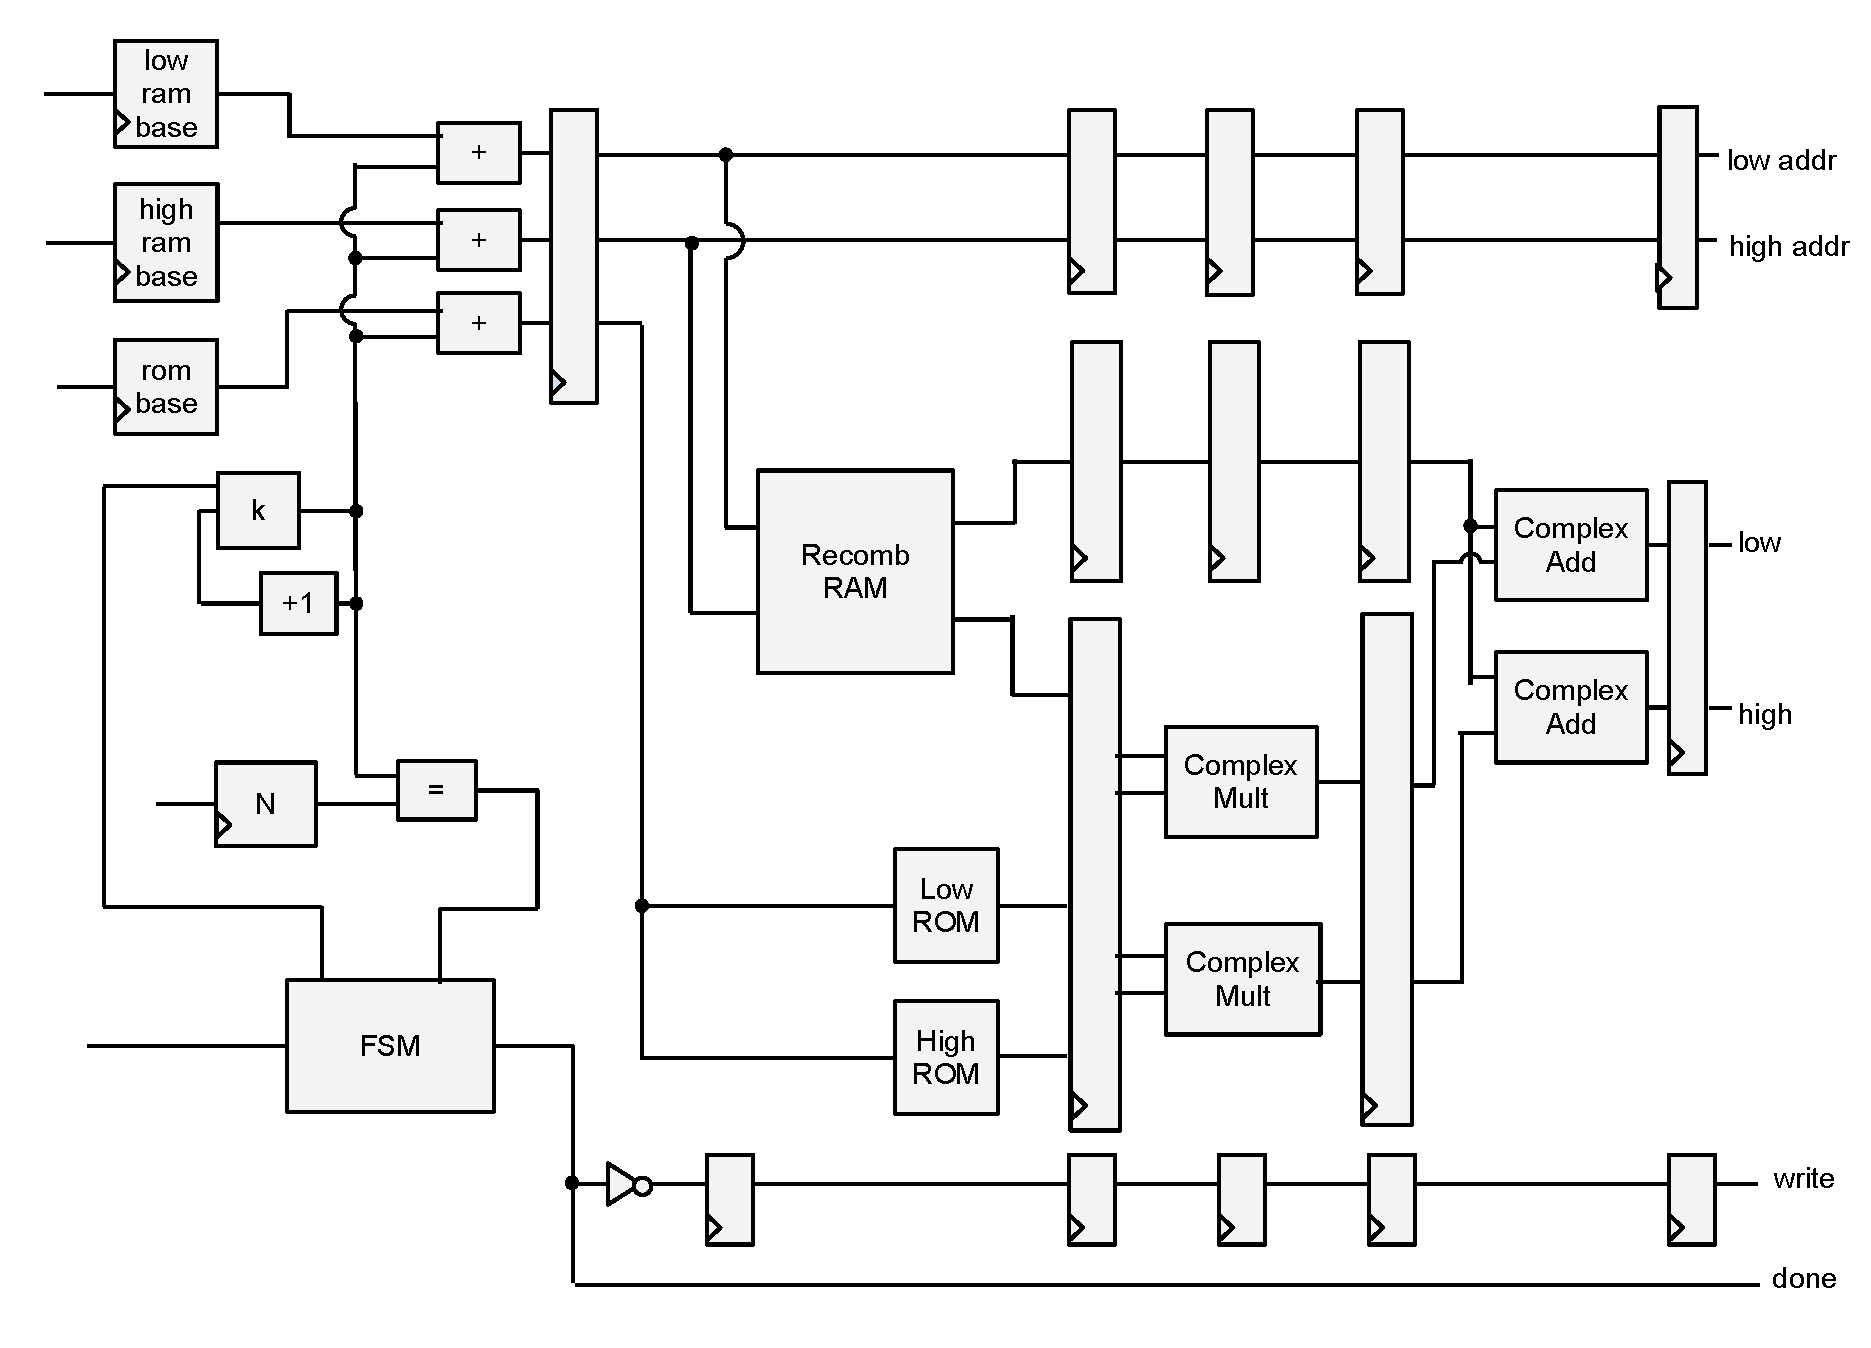
\includegraphics[scale=0.3]{recombinator}
	\caption{Recombination Unit}
\end{figure}

The recombination unit computes 32 parts of the recombinational step 
according to equation 2. The upper and lower parts, \(X_k\) and 
\(X_{k + N / 2}\), are computed in parallel. This allows us to re-use the 
odd term \(e^{-\frac{2\pi j}{N}k} O_k\).

The complex multiplier in the recombination unit performs its computation
in two pipelined steps, as follows.

\begin{figure}[H]
	\centering
	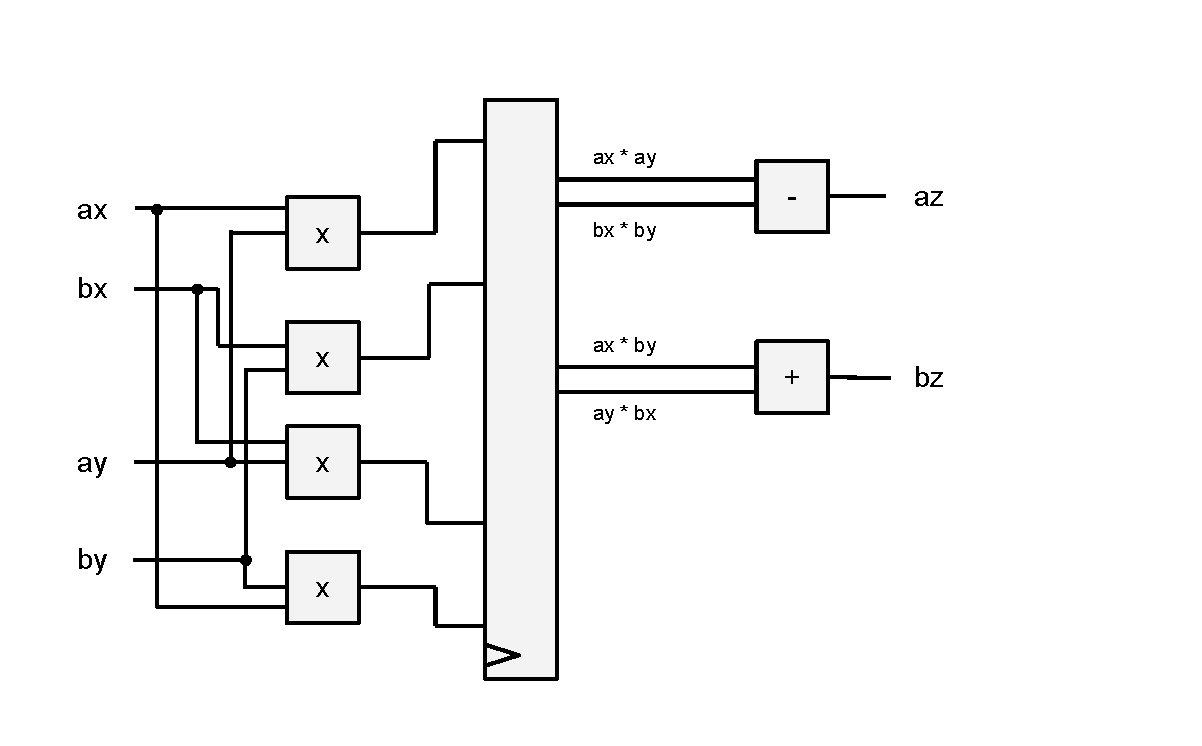
\includegraphics[scale=0.4]{complex-mult}
	\caption{Complex Multiplier}
\end{figure}

Our top-level FFT block uses two DFT units, a recombination unit,
two RAMs (one for time domain data and one for frequency domain data),
four ROMs for the recombination, one ROM for the DFT coefficients, and
a control unit to set all the multiplexers and control the flow of
computation.

\begin{figure}[H]
	\centering
	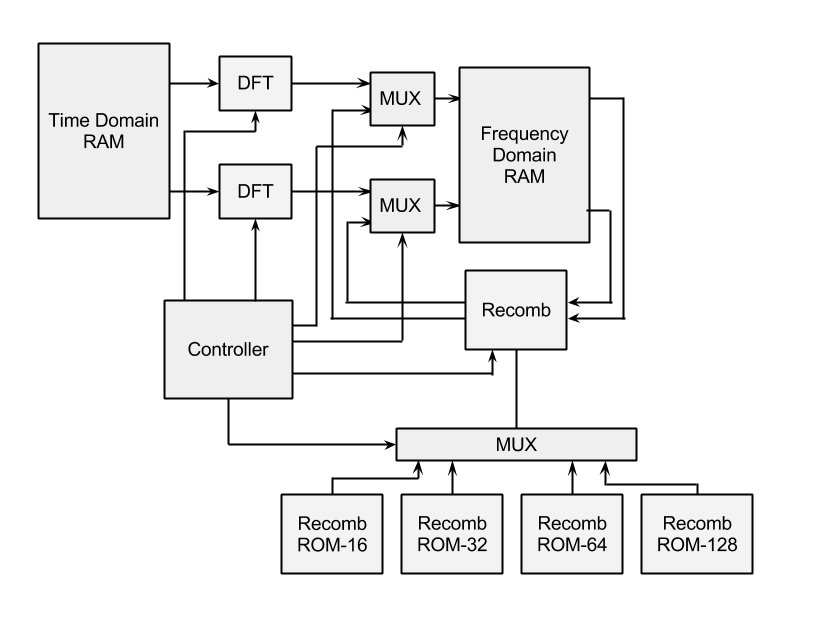
\includegraphics[scale=0.35]{fft-top}
	\caption{FFT Top-Level}
\end{figure}

The DFT ROM holds 256 32-bit values, each one of which represents a
complex number (higher 16 bits for real part and lower 16 bits for
imaginary part). These values represent the constant coefficients
in the DFT equation \(e^{-\frac{2\pi j}{N} n k}\) as 16-bit fixed-point
precision numbers. Each value is addressed by an 8-bit address, where
the highest four bits represent the value of \(k\) and the lowest four bits
represent the value \(n\).

Similarly, the 4 recombination ROMs have 16, 32, 64, or 128 fixed point
imaginary values. These correspond to the constant coefficients
\(e^{-\frac{2\pi j}{N}k}\) from equation 2. The ROMs have 4-bit addresses, 
so only 16 values can be accessed during a single recombination step. 
For the larger ROMs, a select input set by the controller control which 
chunk of 16 values can be addressed.

The controller, in response to an external start signal, triggers
16 DFT computations, with 2 computations running in parallel at a time.
This is followed by 4 stages of recombination. Each recombination stage
uses a different ROM and consists of 8 steps (32 out of 256 outputs are
computed on each step).

The multipliers used in this design all use the dedicated multiplier 
circuitry on the Cyclone II. All RAMs and ROMs use the dual-port M4K
block RAM.
	
\subsection{Audio Buffer}

The audio buffer controls playback of the audio data. It contains a RAM
holding 512 16-bit values and a unit that speaks to the Wolfson WM8731
audio codec on the DE2 board.

\begin{figure}[H]
	\centering
	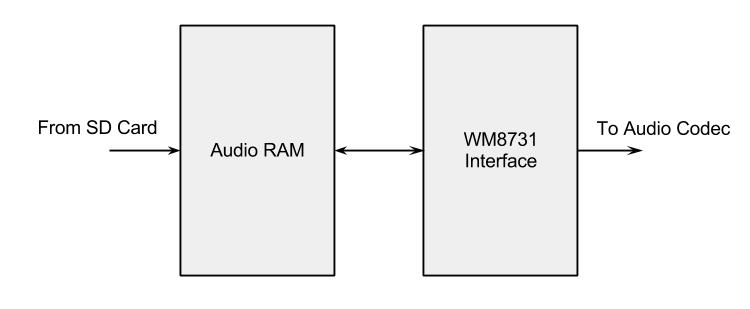
\includegraphics[scale=0.3]{audio-buffer}
	\caption{Audio Buffer}
\end{figure}

The audio codec interface reads in a 16-bit sample from the audio RAM and
transmits the bits serially to the audio codec. Once the last bit has been
transmitted, the next sample is requested from the audio RAM.

The audio RAM is effectively split in two so that the audio codec interface
plays samples from one half while the SD card writes to the other. This is
the reason why the RAM is chosen to hold 512 samples, since one SD card
block is 512 bytes, or 256 samples. Once the audio codec interface plays 
sample 255 or 511 (indexed from 0), it sends a signal indicating that the 
SD card controller should read in another block.

\subsection{Visualizer} 

There are two main tasks that the vizualizer needs to accomplish.  
The first is sequentially reading in the data produced by the FFT and the 
other is displaying that data on the vga.  Originally all 256 different 
frequencies were being displayed however after initial designs the decision 
made was to include data for the first 32 frequencies on the display since 
these are the hearable frequencies.  The reading process requires two states, 
a holding state and a reading state.  The transition to reading happens when 
the FFT sends a "done" signal which means that the data is in place to be read.  
For display purposes, the 32 frequencies are placed into 16 bins, 2 per bin, 
each of which corresponds to one of sixteen bars located horizontally across 
the screen.  The height of these bars is decided by summing the amplitude of 
the two frequencies contained in the bin and then scaling this value to the 
necessary height for the screen.

It was necessary to use two different clocks since the vga display requires a 25.1 MHz clock, in this case a 25 MHz clock as used.  There was no need to read in data on the slower clock and therefore the a 50 MHz clock was used there so as to read the data as quickly as possible. 

An additional functionality that was added was the ability to change color of the bars appearing on the screen.  
Three switches correspond to red, green, and blue and allow the user to mix 
and match to create different colors.  The switches are active low so the 
default color when all switches are "off" is the white so as to be seen on the 
black background.  In order to improve the accuracy of the display adjustments 
were made so that new data is only read in when data is not being drawn to the screen.

\begin{figure}[H]
	\centering
	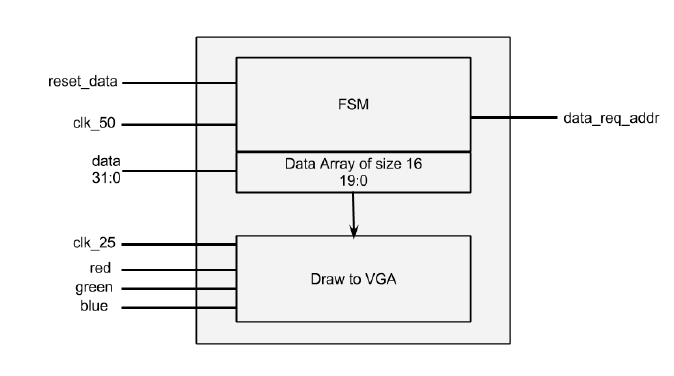
\includegraphics[scale=0.5]{viz_block_diagram.png}
	\caption{Visualizer}
\end{figure}
% timing diagram
% test benches if available

\subsection{SD Card Controller}

The SD card controller is responsible for initializing the SD card's own
built-in controller, sending read commands to the SD card as necessary, and
receiving the data and writing it to the audio buffer.  It takes as inputs the
global clock and a 32-bit SD block address to read, and it sends write data,
write address, and write enable to the audio buffer.

\subsubsection{SPI Bus Protocol}

SD cards support three communication protocols: SPI bus mode, 1-bit SD bus
mode, and 4-bit SD bus mode. Our implementation uses the SPI bus, which is the
simplest; the controller acts as the master device, and the SD card acts as a
single slave.  The signals on the SPI bus are:
\begin{itemize}
	\item SCLK - clock, controlled by the master
	\item MOSI - master out, slave in
	\item MISO - master in, slave out
	\item CS' - chip select (active low)
\end{itemize}

\subsubsection{SD Card Data Formatting}

Support for standard filesystems is not implemented. However, there is support
for multiple song files. SD cards are addressed as 512-byte blocks. As such,
the first 512 bytes of the SD card is dedicated to metadata - it contains the
start addresses for each song on the SD card.

The songs themselves are in 16-bit raw PCM format, written to the SD card end
to end and aligned to 512 byte boundaries. The start addresses of each
song, as discussed earlier, are contained in the metadata block.

\subsubsection{Block Diagram}


% block diagram
% state diagram
% timing diagram
% test benches if available

\subsection{Software User Interface}

\subsection{Miscellaneous Controller Components}
\subsubsection{The Conductor}
\subsubsection{Phase-Locked Loop for Multiple Clocks}

The visualizer unit and audio playback required different clocks to drive their 
respective peripherals, but also required clocks to synchronize communication 
with other modules in the kanto 
. To most easily configure these clocks, 
a Phase-Locked Loop (PLL) was generated from an Altera Megafunction. The PLL 
was used to generate a 50MHz clock for general system synchronization, a 25MHz 
clock to drive the VGA display, and 11.29 MHz for the audio output. 
%% NEED AUDIO CLOCK SPEED 44100/s? 

\section{Timeline \& Milestone Progress}
\begin{tabular}{cc|p{7cm}p{3cm}}
\textbf{Milestone} & \textbf{Date} & \textbf{Goal} & \textbf{Accomplished}\\ \hline
&&&\\
Milestone 1 & Apr 2 & RTL design and block diagrams of all peripherals.&
	\textit{Completed.}\\
&&&\\
Milestone 2 & Apr 16 & Individual peripherals written in VHDL and test benched.&
	\textit{Completed.}\\
&&&\\
Milestone 3 & Apr 30 & Build interfaces between all peripherals and finish synchronization software. &
	\textit{Completed}\\
&&&\\
Deadline&May 15&System complete and presentation finished.&\textit{Completed.}\\
&&&\\
\end{tabular}
%% should include software inclusion somewhere


\section{Contributions \& Teamwork}
	\begin{itemize}
	
	\item
	\textbf{Kavita Jain-Cocks}
		\begin{enumerate}
		\item item
		\item item
		\end{enumerate}
	
	\item 
	\textbf{Howard Mao}
		\begin{enumerate}
		\item item
		\item item
		\end{enumerate}
	
	\item 
	\textbf{Amrita Mazumdar}
		\begin{enumerate}
		\item item
		\item item
		\end{enumerate}
	
	\item 
	\textbf{Darien Nurse}
		\begin{enumerate}
		\item item
		\item item
		\end{enumerate}
	
	\item 
	\textbf{Jonathan Yu}
		\begin{enumerate}
		\item item
		\item item
		\end{enumerate}
	
	\end{itemize}

\section{Challenges \& Lessons Learned}

\subsection{Changing Parallelism Levels}

At a certain point in a project, we had to reduce the amount of parallelism in 
the FFT unit in order to reduce the number of logic gates used by the board. 
We found that reducing the level of parallelism is often just as hard, if not 
harder, than adding parallelism. Both require extensive changes. It would have 
made things much easier if we had decided on the proper level of parallelism 
at the outset. If we had done some quick calculations at the outset, we would 
have discovered that could have used a very low level of parallelism and still 
been well within the deadlines imposed by the timing of our system.

\subsection{Timing Issues}

Timing issues can be a big problem in a complex design, especially if external 
hardware is involved, as different hardware peripherals require different clocks. 
For our design, the audio codec used a 11.29 MHz clock, the VGA used a 25 MHz 
clock, and the SD card used a 6.25 MHz clock. We used a PLL for the first two 
and clock enables for the last one (since the SD card clock wasn’t always running). 
But passing status and control signals between units running on different clocks 
ended up being a minor challenge. We ended up solving this problem by either 
stretching the signals or detecting the rising edge of signals.

The fact that both reading in VGA data and refreshing the VGA display take more 
than one cycle means that we needed to ensure that the data wasn’t being changed 
while the display was in the middle of refreshing. This was accomplished by 
reading data into a separate set of registers and only transferring it to the 
registers used by the refreshing process once the refresh had reached the edge 
of the screen.  This made it possible to reduce the flickering that was being 
seen on the display.

\subsection{Interfacing to External Hardware}

Interfacing to external hardware like the SD card and the audio codec were by 
far the most challenging parts of the assignment, mainly because it was very 
difficult to debug. Since proper functioning depended on what the external 
hardware was doing, we couldn’t really use VHDL testbenches like we did for 
the rest of the components, since our testbenches wouldn’t exactly replicate 
the behavior of the external hardware. We found that the best way to get 
interfaces to external hardware working was to base our implementation off of 
existing implementations. For instance, for the audio buffer, we used the 
components provided for lab 3 to interface with the audio codec, but modified 
the files to achieve the correct sampling frequency. For the SD card controller, 
we based a lot of our code off of the SPI controller from Prof. Edward’s Apple 
II FPGA project, as well as the SD card driver code in the Linux Kernel. 

\subsection{Reduction of Hardware Usage}

At its peak, our design used up 89\% of the logic elements on the FPGA. 
We found out that this was because we were accidentally using logic elements 
instead of block RAM for all of our memory components. After switching over 
the memory components to block RAM, our logic element usage went down to only 
10\%, while our block ram usage went from 1\% to only 5\%. This showed us the 
importance of actually using memory elements for memory.

Changing things over to block RAM did require a lot of other changes to our 
design. For instance, since the block RAM only had two ports, we had to 
dramatically reduce the amount of parallelism in the FFT unit. We also had to 
duplicate some memory. For instance, whereas before, the FFT unit and audio 
buffer shared the same memory for the time domain samples, we eventually had 
to separate this into two different RAMs which the SD card controller wrote 
two simultaneously. However, as mentioned above, this duplication did not add 
that much to our memory requirements. 

Having a modular design, both at the highest level and at the level of each 
component, made these changes go relatively smoothly.

\section{Reflections \& Prospectus}

Our group is very satisfied with the final version of our project.  
Although certain elements did not conform to the originally decided-upon 
structure - for example, the SRAM was replaced with block RAM, and the software 
played a different role than was originally foreseen - we did accomplish all 
major project goals and added slight additional functionality such as 
changeable colors on the visualizer and track selection.

Our plan for completion of the project consisted of each component being 
developed and tested individually and then linked together. Although this plan 
did not end up backfiring in this particular case, an alternate method could 
have been a more step-by-step approach, starting with the SD card and moving 
“linearly” through the different components ending with the visualizer. This 
method would have allowed us to have more concrete deliverables during 
milestones as well as to have a more exact knowledge of exactly where we were 
in the process.

Another consequence of our scheduling was that, as the semester progressed, 
we discovered that, although we remained fairly on track with our predetermined 
milestones throughout the semester and completed the project ahead of the 
deadline, our description of them was slightly vague and hard to verify during 
the biweekly milestone check-ins. This could have been remedied in multiple ways. 
One option would have been to decide upon specific deliverables due at each 
milestone to demonstrate our progress. Another would have been to review our 
milestones with Professor Edward or our adviser before deciding upon them.

One situation that needed to be contended with was that we had a fairly large 
group and also lost a group member early in the process.  That being said, 
we felt that by staying organized and updating the entire group regularly on 
our progress we were able to stay on track and informed about the status of the 
project and what needed to be accomplished next as well as compensate for the 
lost group member.

Although all the initial project goals have been accomplished, there are still 
a few possible improvements and new features that could be implemented.
For instance, the visualization could be made more complex than simply 
displaying bars for each frequency. Having a more interesting visualization 
would vastly improve the "coolness" factor of our project. Another possible 
improvement would be to change the SD card format from our custom format to a 
standard FAT filesystem. This would make it easier for the user to add songs to 
the SD card, as they could simply copy audio files to the filesystem instead of 
having to use custom tools for converting the data and writing it to the block 
device.
 
 \appendix
\section{Source Code}
 \subsection{VHDL}
 \subsection{C}
 \subsection{Python} %should we include python scripts to generate things? eh
 
\end{document}
